\chapter{Implementation}
\label{chap:implementation}
This has the description of how you actually went about implementing the project.  This should be focused on the interesting challenges and how those related to the project.

\section{Creating line of sight using the stencil buffer}
\subsection{Creating the view mesh}
The first step of creating the line of sight is the field of view mesh. This mesh is created by casting rays from the player position with a certain angle step between. The distance between each angle step is determined by a mesh resolution variable multiplied with the view angle.

\section{Providing a responsive user experience for clients while using a mostly server authoritative model}
\subsection{Adding consistent force for server/clients}
\label{sec:conForce}
A rather common component to work with in Unity is rigidbodies. These are used for any physics based movement and are generally something you would like to keep synchronised across the network as well. Rigidbodies are synchronised by the NetworkTransform component and while one might believe that applying force to the rigidbodies in this case would keep them consistently synchronised across the network, this is actually not the case. In the case of trying to apply force from the player's position towards a point, the server player will experience a stronger amount of force than the clients will. In the case of a peer to peer based game like Dockit League, this is unwanted behaviour as the server and clients should experience the same or very similar forces.

We tried a couple of different workaround like synchronising the code for adding force through the use of ClientRpc's or increasing the synchronisation rate of the rigidbodies, but none of these ended up being a usable solution. The issue in general is a result of calculating force vectors on the server based on player positions. This does not necessarily work as by the time the code executes on the clients, their new and updated positions have changed enough to make the force direction incorrect. We ended up trying to use TargetRpc's as a workaround and send the strength of the force, the force mode and the position we wanted to add force towards as parameters. Using this approach allowed the player to locally calculate the force vector and provided far more consistent results than any previous approaches. 

\section{Working around Unity's networking limitations}
    - Unity's networking systems have their limitations
    - Command, ClientRPCs and so on are not able to return data. They cannot take components as parameters, they cannot be overloaded, they do not support generics/templates.
    - Calling any commands requires authority. Only the player object has this. 
    
    - Using [ServerCallback] or checking for docking.isServer in any collision callbacks to make them only happen on the server. 

\subsection{Providing network spawned objects with references to their owners and vice versa}
    - There are cases where the player needs to have a reference back to its spawned object and vice versa if they affect each other. 
    - TargetRPCs in combination with interfaces. 

\subsection{Allowing abilities to use network functionality while still being MonoBehaviour's without any authority}
    - Going through docking to do any synchronized code. 

\section{Using Coroutines for interpolation}
    - Nice for quick interpolations you simply want to start without any additional code in update loops and what not. 
    - Not fully linear. Slows down by the end, in case that is of importance. 

\section{Using Unity to control programmatic interpolations}
\label{sec:boomerangCurve}
Unity as a game engine already has fairly robust and powerful animation tools that allows the developer to create and manage animations directly in the editor. These animation tools have a lot of versatility, but there are times where the developer might want a bit of extra control and use a programmatic interpolation instead. 

In our case we needed to produce a curve for a boomerang to travel through while developing the boomerang kit. We decided to perform this interpolation through the use of a Cubic Bezier curve as these curves are flexible, very simple to control and can provide a nice squeezed arc for the boomerang to interpolate through. Another option would be to use a Hermite curve, but we ended up sticking with Bezier curves as it would make the code more readable for all group members due to everyone's preexisting familiarity with these. The formula for interpolating through Cubic Bezier curves is as follows:
$$
B(t) = (1 - t)^3 P0 + 3(1 - t)^2 t * P1 + 3(1 - t)t^2 * P2 + t^3 P3 
$$
The function takes five parameters:
\begin{description}
    \item[P0:] The start position of the curve
    \item[P1:] The handle of the start position
    \item[P2:] The handle of the end position
    \item[P3:] The end position of the curve
    \item[t:]  The input time of the interpolation. Has to be in range [0, 1]
\end{description}

We use the Bezier Curve in two ways:
\begin{enumerate}
    \item To create vertices for a LineRenderer component that displays the approximate travel path of the boomerang while holding down the ability button
    \item To interpolate the boomerang itself as the ability button is released
\end{enumerate}
When we say approximate path we mean the path that the boomerang would travel if the player stood perfectly still.
The point of displaying an approximate path is to give the player an idea of how far the boomerang will travel before returning. It is generated using local coordinates rather than world coordinates. On the other hand, actually throwing the boomerang stores the world position of both handles while using current position of the player as start and end point. This means that the bezier curve will dynamically change based on how the player is moving, but still travel to the peak of the approximate path.  

While the Bezier Curve is nice for providing a curve to interpolate through, the animation itself looked fairly uninteresting as the change in \textbf{\textit{t}} was linear due to the fact that we simply used a timer variable for it. The boomerang kit's abilities are built around the position of the boomerang so we needed to provide ample time for the player to use the kit's abilities as the boomerang approached the peak of its curve. 

\subsection{Handling the velocity of the animation}
While developing, we drew several graphs that could represent a non linear change in our input parameter \textbf{\textit{t}}, but were unsure of how we could get representations of these into our code.  This section includes two different ways of providing graphs that can be evaluated by the game to control the velocity of the animation.

The first solution we found by looking at Unity's documentation was to use Unity's built in AnimationCurve~\cite{unityDocumentationAnimationCurve} type. AnimationCurves can be public members of any MonoBehaviour class, allowing the developer to use the inspector to generate curves in the range of [0, 1] for both axes by default. These curves also have an evaluation function that allows the developer to provide a input time parameter and get an output back. 

In our case, we wanted the boomerang to accelerate from the start, decelerate towards the halfway point of the animation and then accelerate again towards the end. This was fairly simple to implement using the AnimationCurve type since it works in the range of [0, 1] by default. All we needed to do was to provide the evaluation function a time variable and use its output as \textbf{\textit{t}} into the Bezier Curve interpolation. 
    
\begin{figure}[tbph]  %t top, b bottom, p page | you can also use h to try to get the figure to appear at the current location
  \centering
  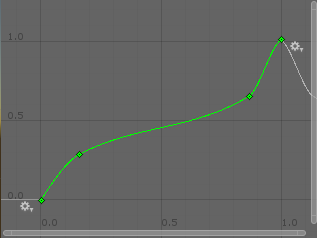
\includegraphics[width=.5\textwidth]{images/BoomerangAnimationCurve}
  \caption[Boomerang animation curve using Unity's built in type]{This curve shows the change in \textbf{\textit{t}} as time goes from 0 to 1 on the x axis using Unity's AnimationCurve type.}
  \label{fig:boomerangcurve0}
\end{figure}

\begin{figure}[tbph]
    \centering
    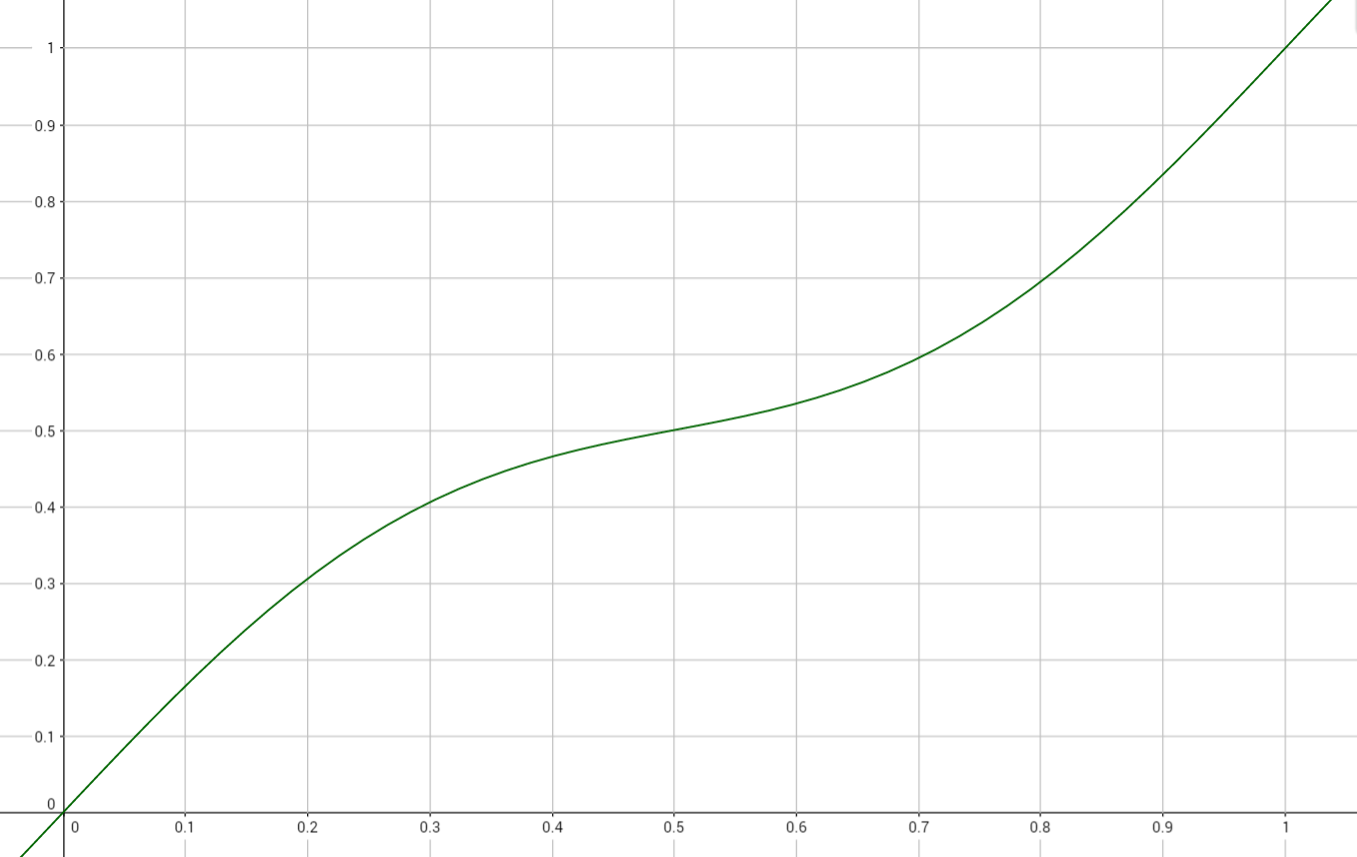
\includegraphics[width=.5\textwidth]{images/BoomerangMathematicalCurve}
    \caption[Boomerang curve using a mathematical formula]{This curve shows the change in \textbf{\textit{t}} as time goes from 0 to 1 on the x axis using the mathematical curve $f(x) = x + sin(6.28x) / 9$}
    \label{fig:boomerangcurve1}
\end{figure}
    

As seen in Figure~\ref{fig:boomerangcurve0}, the AnimationCurve approach provides an easy to use interface with control points and control point handles, but there is also another way of solving the problem. 

A more generic approach would be to use a mathematical function like $f(x) = x + sin(x) / c$ to create a similar looking curve, but this approach has some problems that need to be dealt with. First of all, the curve needs to be scaled so that the wanted part of it is within the range of [0, 1] for both axes in order for the output to work with the interpolation function. This could be achieved by playing around with a graph plotting tool like GeoGebra or similar. In our case, the function $f(x) = x + sin(6.28x) / 9$ as seen in Figure~\ref{fig:boomerangcurve1} would provide similar behaviour to Figure~\ref{fig:boomerangcurve0}, but still lack the strong acceleration towards the end of the interpolation. This approach gives less control to the developers who work in the engine and spending time trying to scale the curves can be quite time consuming.

We also made sure to check the performance difference between the two approaches by measuring the execution time of both. We measured the time spent on each function per update and averaged out the time values after 10 boomerang throws. This gave us the following results:

\begin{itemize}
    \item The average execution time of the AnimationCurve's evaluation function took \textasciitilde$ 0.36 \mu s$
    \item The average execution time of the math function took \textasciitilde$ 0.20 \mu s$.
\end{itemize}

The time difference was calculated using Unity's Time.realTimeSinceStartup variable. The Time.realTimeSinceStartup float is measured in seconds so we multiplied the average time difference by $10^6$ and used a output precision of two decimals for these results. 
The mathematical approach provides a small increase in performance as seen from the results, but in our case the difference is too small to warrant using it. The AnimationCurve approach is far easier to work with directly in the editor instead of using external graph tools to modify the curve to our needs. On the contrary, the mathematical approach is more generic and might see use in non Unity applications.

\section{Balancing in preparation for user testing}
The full game functionality required for proper user testing ended up being implemented rather late into the project's development. Due to this we had limited time for user testing and needed to provide the testers with a build that already had some initial balancing done. 
Dockit League is an asymmetrical game due to the variety of available docking kits so we used a mathematical model~\cite{schell2014art} for the initial balance iteration. Doing so allowed us to have a overview over the different kits including their strengths and weaknesses.

\begin{table}[tbph]
\centering
\caption{Initial balance table}
\label{tab:initBalance}
\begin{tabular}{@{}llllll@{}}
\toprule
\textbf{Docking Kit} & \textbf{Health} & \textbf{Movement Speed} & \textbf{Damage} & \textbf{Utility} & \textbf{Totals} \\ \midrule
Boomerang Kit        & Low (1)         & High (3)                & High (3)        & Medium (2)       & 9               \\
Brawler Kit          & High (3)        & Low (1)                 & Medium (2)      & Medium (2)       & 8               \\
Bomber Kit           & Medium (2)      & Low (1)                 & High (3)        & Medium (2)       & 8               \\
Marksman Kit         & Medium (2)      & Medium (2)              & Medium (2)      & Medium (2)       & 8               \\
Sniper Kit           & Medium (2)      & Medium (2)              & High (3)        & Medium (2)       & 9               \\
Tank Kit             & High (3)        & Low (1)                 & Low (1)         & High (3)         & 8               \\
Trapper Kit          & Medium (2)      & Medium (1)              & Low (1)         & High (3)         & 8               \\
Support Kit          & Medium (2)      & Medium (2)              & Low (1)         & High (3)         & 8               \\ \bottomrule
\end{tabular}
\end{table}

The balance table~\ref{tab:initBalance} contains columns for kit name, kit health, kit movement speed, damage and utility. The damage column has values assigned based on the potential damage output of the kit while the utility column has values assigned based on the overall the utility the kit provides through its abilities. This includes abilities that apply modifiers and other effects without necessarily focusing on damage. Further tweaking on cooldowns, damage values and modifier durations is the focus of the user testing section rather than the initial balancing as this section is supposed to give a rough estimate of each kit's capabilities. 
Additional information on the various docking kits and their abilities can be found in section~\ref{sec:dockingKits}

\subsection{Observations from the initial balance table}     
As seen in table~\ref{tab:initBalance}, the sniper and boomerang kits end up with a slightly higher total than the other kits. This is a deliberate decision as both kits have a high damage potential if played well while having a low to medium damage potential otherwise. We believe that both kits are fairly challenging to play in order to achieve their full damage potential so the difficulty offsets the the fact that the two kits are a bit stronger than the rest. 
The boomerang kit requires the player to hit with multiple boomerangs while they move forwards and then again once they move back for the maximum amount of damage. The sniper kit requires time and preparation before shooting and rewards a large amount of damage if the projectile actually connects.  
These parts of the two kits allows us to provide a high risk, high reward ratio for playing well.

An interesting thing to note with our current design is that none of the implemented kits have a low utility value. All the kits feature at least 2 abilities that provide utility through either the use of modifiers or other effects. The utility abilities for the kits are generally designed to help patch up the weaknesses of each kit. The brawler kit for example struggles fighting ranged enemies due to its low speed and melee weapon, but contains abilities for reflecting projectiles and stunning opponents to get closer. If any future development were to take place on the project, creating kits with less utility and a larger focus on the other statistics could improve the variety of of the kits.

One important aspect of game balance is the fact that distinct weaknesses is a great way to provide counterplay and avoiding dominant strategies~\cite{gameBalanceWeaknesses}. While the kits generally have abilities that help them somewhat with their weaknesses, these abilities have long enough cooldowns to not always be available. Balancing cooldowns isn't the only way to exemplify the weaknesses of kits though. 
The boomerang kit is the only kit with low health and has a large damage potential with high movement speed. One of the weaknesses of the boomerang kit is the low health and being caught unaware by enemy players will lead to a swift death. The limited field of view also helps creating situations where the player might have been inattentive and not seen an enemy sneaking in from behind. The high speed of the kit might be seen as beneficial, but can result in the player carelessly rushing into enemies who are right around the corner of walls and other obstacles. 